\documentclass[a4paper,12pt]{article}
\usepackage[utf8]{inputenc}
\usepackage{geometry}
\usepackage{graphicx}
\usepackage{amsmath}
\usepackage{hyperref}
\usepackage{fancyhdr}
\usepackage{listings}
\usepackage{xcolor}
\usepackage{float}

% Configurando margens de 2 cm
\geometry{
  a4paper,
  left=1.5cm,
  right=1.5cm,
  top=2cm,
  bottom=2cm
}

% Configurando o cabeçalho
\pagestyle{fancy}
\fancyhf{}
\fancyhead[L]{Exercise TD - Plate-Forme Sociale}
\fancyfoot[C]{\thepage}

% Criando a capa
\begin{document}
\begin{titlepage}
    \centering
    {\LARGE \textbf{Exercise TD - Plate-Forme Sociale}}\\[1.5cm]
    
    \textbf{Name:} João Pedro Marçal Storino \\[0.5cm]
    \textbf{Course:} ICM 2A \\[0.5cm]
    \textbf{Subject:} Informatique - Software Engineering \\[0.5cm]
    \textbf{Date:} \today \\[2cm]
    
    \vfill
    
    \textbf{Université Mines Saint-Étienne} \\[0.5cm]
    \textbf{Academic Year:} 2024
\end{titlepage}

\newpage
\tableofcontents
\newpage

\section*{Introduction}

This document presents a complete architectural study and analysis for a social platform application. The goal was to approach the system design using multiple methods to enhance learning and provide a deeper understanding of software architectures. The methods include:

\begin{itemize}
    \item \textbf{Component-Based Architecture:} Defining system components, their responsibilities, interfaces, and dependencies.
    \item \textbf{Architectural Styles:} Exploring two major architectural styles – \textbf{Pipe-and-Filter} and \textbf{Blackboard} – to demonstrate flexibility and scalability.
    \item \textbf{Microservices Architecture:} Implementing a modular design inspired by the DeathStarBench project, utilizing Apache Thrift for high-performance RPC communication.
    \item \textbf{Modeling Diagrams:} Component, Sequence, and Deployment diagrams were created to visualize the architecture and workflows.
\end{itemize}

This approach provides a structured methodology for system design while enabling adaptability for new functionalities, such as URL shortening and hashtag support. Each architecture was analyzed to evaluate the impact of these changes, with conclusions drawn regarding their advantages and trade-offs.

\newpage
\section{System Architecture for Social Platform}

\subsection{Application Components}

The components of the social platform and their roles are detailed below:

\begin{itemize}
    \item \textbf{AuthService (Authentication Service):}
    \begin{itemize}
        \item \textit{Responsibilities:} Manages user authentication, including login and registration.
        \item \textit{Interfaces:} Exposes endpoints for login and registration.
        \item \textit{Dependencies:} Requires access to the \textbf{Database} for user validation.
    \end{itemize}
    
    \item \textbf{ContentService:}
    \begin{itemize}
        \item \textit{Responsibilities:} Handles creating, reading, updating, and deleting posts.
        \item \textit{Interfaces:} CRUD endpoints for posts.
        \item \textit{Dependencies:} Requires \textbf{AuthService} for user validation and \textbf{MediaService} for media uploads.
    \end{itemize}

    \item \textbf{MediaService:}
    \begin{itemize}
        \item \textit{Responsibilities:} Manages media files (images and videos), including storage and retrieval.
        \item \textit{Dependencies:} Interacts with a file storage system (e.g., AWS S3).
    \end{itemize}

    \item \textbf{HistoryService:}
    \begin{itemize}
        \item \textit{Responsibilities:} Retrieves a user's post history.
        \item \textit{Dependencies:} Queries post data from the \textbf{Database}.
    \end{itemize}

    \item \textbf{RecommendationService:}
    \begin{itemize}
        \item \textit{Responsibilities:} Provides personalized recommendations for users to follow.
        \item \textit{Dependencies:} Requires user activity data and \textbf{SubscriptionService}.
    \end{itemize}

    \item \textbf{SearchService:}
    \begin{itemize}
        \item \textit{Responsibilities:} Searches for posts or users based on keywords.
        \item \textit{Dependencies:} Accesses indexed data from the \textbf{Database}.
    \end{itemize}

    \item \textbf{SubscriptionService:}
    \begin{itemize}
        \item \textit{Responsibilities:} Handles follow/unfollow actions for users.
        \item \textit{Dependencies:} Updates and queries connections in the \textbf{Database}.
    \end{itemize}

    \item \textbf{Database:}
    \begin{itemize}
        \item \textit{Responsibilities:} Centralized storage for users, posts, media metadata, and subscriptions.
    \end{itemize}
\end{itemize}

\subsection{Connectors Between Components}

The following connectors facilitate communication between the components:

\begin{itemize}
    \item \textbf{REST API:} Allows synchronous communication for actions like login, post creation, and search queries.
    \item \textbf{RPC (Remote Procedure Call):} Enables efficient inter-service calls, such as media upload or recommendation fetch.
    \item \textbf{Asynchronous Messaging:} Manages notifications and background updates using message queues (e.g., RabbitMQ).
    \item \textbf{Database Connector:} Ensures consistent access to data for all components.
    \item \textbf{File Storage System:} Stores and retrieves large media files for posts.
\end{itemize}

\subsection{Component Diagram}

Figure~\ref{fig:component-diagram} illustrates the high-level architecture, showing how components interact with one another.

\begin{figure}[H]
    \centering
    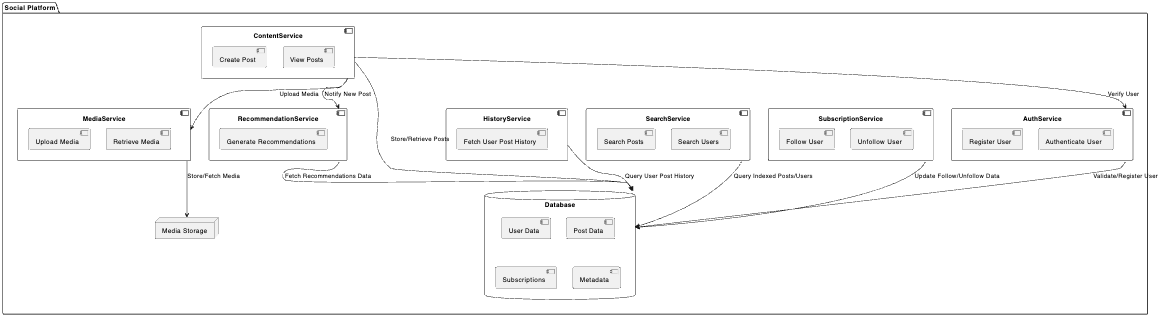
\includegraphics[width=1\linewidth]{UML_component.png}
    \caption{Component Diagram for Social Platform}
    \label{fig:component-diagram}
\end{figure}

\subsection{Dependencies Between Components}

The following dependencies exist:

\begin{itemize}
    \item \textbf{AuthService} requires the \textbf{Database} to validate users.
    \item \textbf{ContentService} depends on \textbf{AuthService} for user authentication and \textbf{MediaService} for handling media.
    \item \textbf{RecommendationService} retrieves user activity and subscription data.
    \item \textbf{HistoryService} queries user post data from the \textbf{Database}.
\end{itemize}

\subsection{Sequence Diagram: Full Platform Workflow}

The sequence diagram in Figure~\ref{fig:sequence-diagram} represents the complete workflow, including registration, login, post creation, media uploads, and user interactions.

\begin{figure}[H]
    \centering
    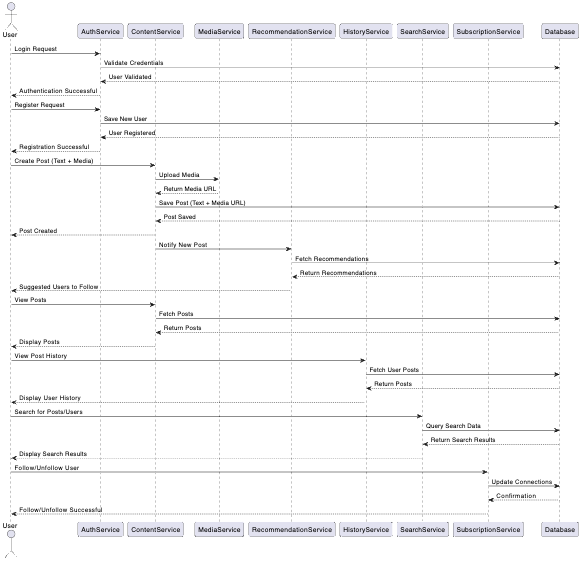
\includegraphics[width=0.9\linewidth]{UML_1.png}
    \caption{Sequence Diagram for Full Platform Workflow}
    \label{fig:sequence-diagram}
\end{figure}

\section{Architectural Styles}

\subsection{Pipe-and-Filter Architecture}

The \textbf{pipe-and-filter} architecture processes data sequentially through independent filters. Each filter performs a specific task and passes the output to the next filter.

\begin{figure}[H]
    \centering
    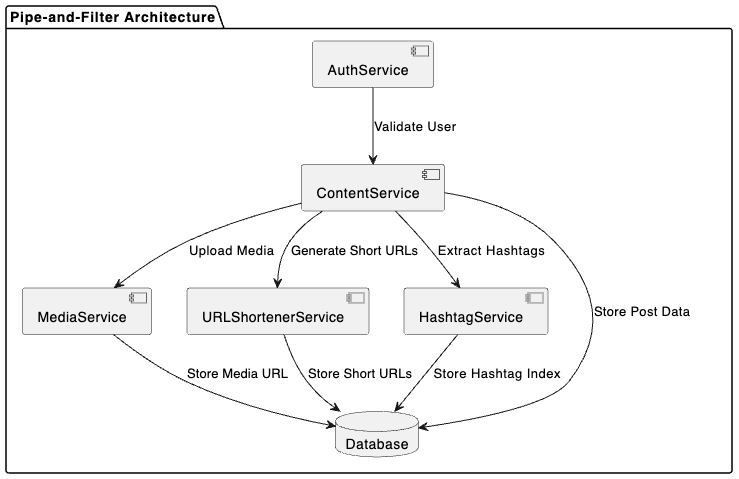
\includegraphics[width=.75\linewidth]{pipe_filter_architecture.png}
    \caption{Pipe-and-Filter Architecture}
    \label{fig:pipe-filter}
\end{figure}

\subsection{Blackboard Architecture}

The \textbf{blackboard} architecture uses a shared data space for interaction among components. Components publish and retrieve information from the blackboard independently.

\begin{figure}[H]
    \centering
    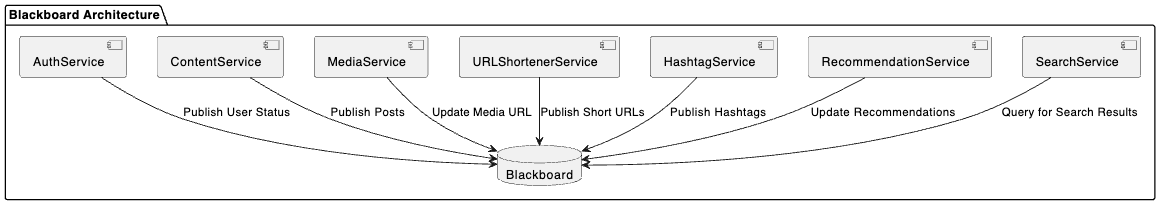
\includegraphics[width=1\linewidth]{blackboard_activity.png}
    \caption{Blackboard Architecture}
    \label{fig:blackboard}
\end{figure}

\subsection{Impact of New Functionalities}

The new functionalities added are:

\textbf{URL Shortening Service:} Generates and redirects shortened URLs.

\textbf{Hashtag Support:} Allows indexing and searching of hashtags. \\

\textbf{Impact Analysis:}
\begin{itemize}
    \item \textbf{Pipe-and-Filter:} Requires modifying the pipeline and adding filters. \textbf{3 components affected}.
    \item \textbf{Blackboard:} New services integrate smoothly with minimal changes. \textbf{2 components affected}.
\end{itemize}

\textbf{Conclusion:} The blackboard architecture is more adaptable for new features due to its flexibility and minimal impact on existing components.

\section{Microservices Architecture}

A microservices architecture, inspired by the \textbf{DeathStarBench} project, has been proposed to implement the social platform. The DeathStarBench social network application utilizes \textbf{Remote Procedure Call (RPC)} as the primary communication method, implemented using the \textbf{Apache Thrift} framework. The architecture leverages REST-like principles to ensure efficient and modular service interactions.

\subsection{Apache Thrift Overview}

Apache Thrift is a framework for scalable cross-language communication. It allows services to define their APIs and data structures using a simple \texttt{.thrift} file, which is then compiled into multiple programming languages. The key features include:
\begin{itemize}
    \item \textbf{Cross-Language Support:} Services implemented in different languages can seamlessly interact.
    \item \textbf{High-Performance RPC:} Enables efficient inter-service communication with minimal overhead.
    \item \textbf{Interface Definition Language (IDL):} Facilitates the definition of APIs and their associated data structures.
\end{itemize}

For this platform, the \texttt{social\_network.thrift} file defines the microservices required for the system, including endpoints for user authentication, post creation, and search functionality.

\subsection{Reconstructed Component Diagram}

Figure~\ref{fig:microservice-components} represents the microservices architecture based on the DeathStarBench model.

\begin{figure}[H]
    \centering
    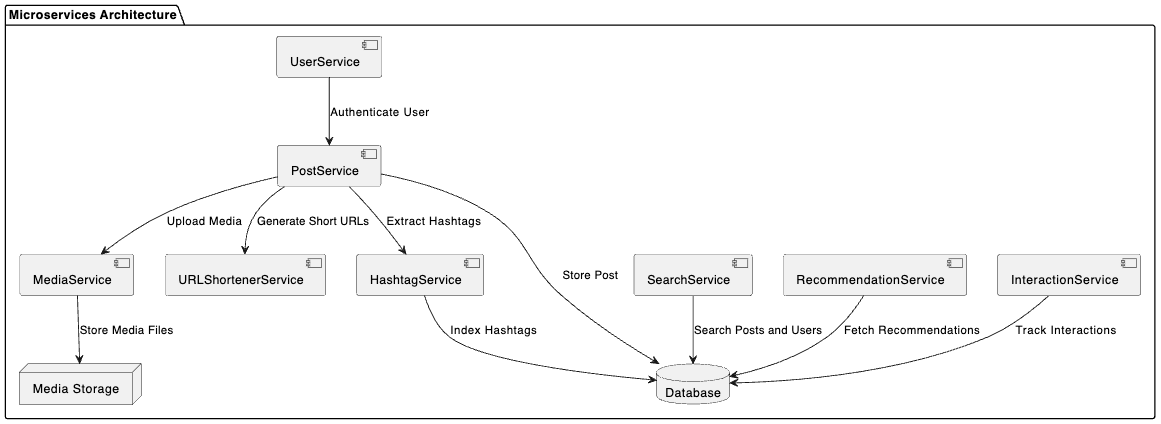
\includegraphics[width=1\linewidth]{microservice-component.png}
    \caption{Microservices Component Diagram for Social Platform}
    \label{fig:microservice-components}
\end{figure}

The architecture consists of the following microservices:

\begin{itemize}
    \item \textbf{UserService:} Handles user registration, login, and authentication.
    \item \textbf{PostService:} Manages CRUD operations for posts.
    \item \textbf{MediaService:} Handles media uploads, retrieval, and storage.
    \item \textbf{SearchService:} Enables searching for posts, users, and hashtags.
    \item \textbf{RecommendationService:} Generates personalized user-following recommendations.
    \item \textbf{URLShortenerService:} Generates and manages shortened URLs.
    \item \textbf{HashtagService:} Extracts, indexes, and stores hashtags.
    \item \textbf{InteractionService:} Tracks likes, comments, and interactions.
\end{itemize}

\subsection{Sequence Diagram}

The sequence diagram (Figure~\ref{fig:microservice-sequence}) outlines the interactions between the microservices for a post creation workflow with media upload and hashtag indexing.

\begin{figure}[H]
    \centering
    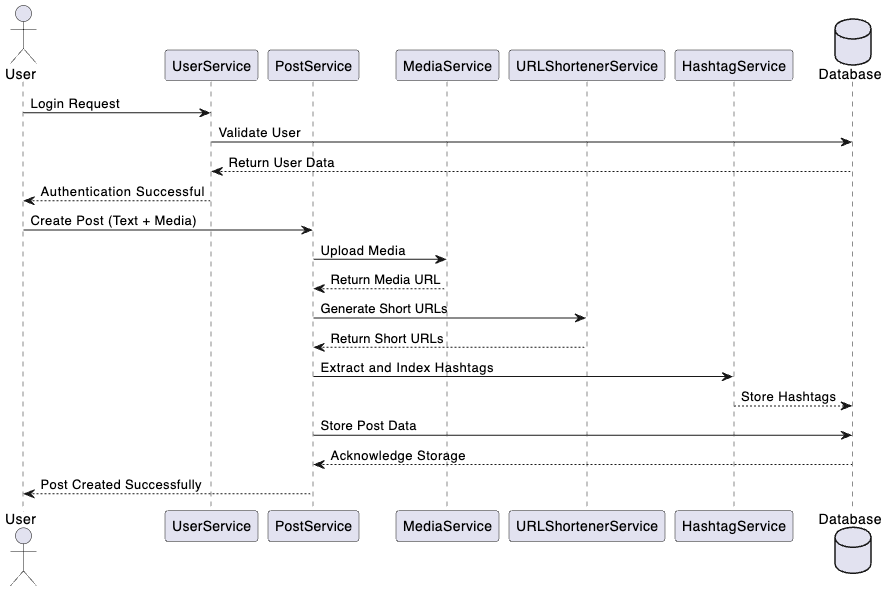
\includegraphics[width=0.9\linewidth]{microservice_sequence.png}
    \caption{Microservices Sequence Diagram: Post Creation Workflow}
    \label{fig:microservice-sequence}
\end{figure}

\textbf{Workflow Steps:}
\begin{enumerate}
    \item \textbf{UserService:} Authenticates the user.
    \item \textbf{PostService:} Receives the new post request and validates data.
    \item \textbf{MediaService:} Uploads media files and provides a media URL.
    \item \textbf{URLShortenerService:} Generates shortened URLs for external links.
    \item \textbf{HashtagService:} Extracts hashtags and indexes them for search.
    \item \textbf{PostService:} Stores the final post in the database.
    \item \textbf{RecommendationService:} Updates recommendations based on the new post.
\end{enumerate}

\subsection{Deployment Diagram}

Figure~\ref{fig:microservice-deployment} shows the deployment model for the microservices architecture.

\begin{figure}[H]
    \centering
    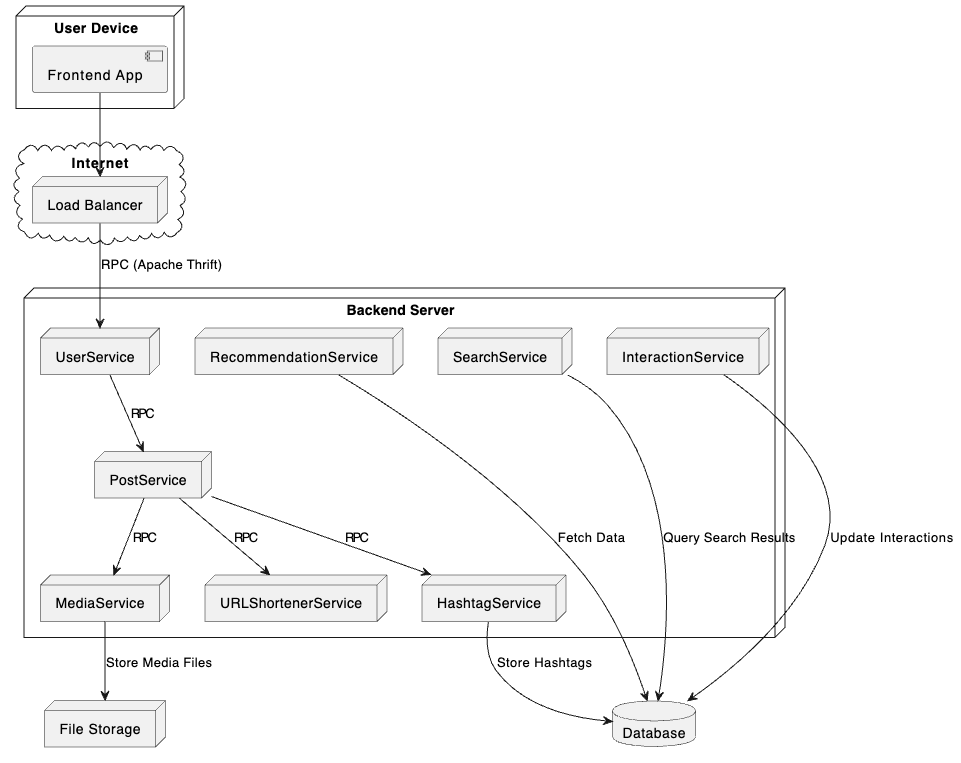
\includegraphics[width=0.9\linewidth]{microservice_deployment.png}
    \caption{Microservices Deployment Diagram}
    \label{fig:microservice-deployment}
\end{figure}

\textbf{Deployment Details:}
\begin{itemize}
    \item Each microservice runs in its own container (e.g., Docker).
    \item Services communicate via RPC over HTTP using Apache Thrift.
    \item A centralized database stores all persistent data.
    \item Media files are stored in an external file system (e.g., AWS S3).
\end{itemize}

\section{Conclusion}

In this document, we explored the architectural design of a social platform application, integrating various approaches to provide a comprehensive solution. The key insights include:

\begin{itemize}
    \item \textbf{Component-Based Architecture:} A clear definition of components, their responsibilities, and dependencies was provided, ensuring modularity and reusability.
    \item \textbf{Pipe-and-Filter vs Blackboard Styles:} Both architectural styles were analyzed, demonstrating the trade-offs between sequential processing (Pipe-and-Filter) and flexibility through a shared data space (Blackboard).
    \item \textbf{Microservices Architecture:} Inspired by DeathStarBench, the microservices design provided scalability, modularity, and high performance using Apache Thrift RPC.
\end{itemize}

We further evaluated the impact of new functionalities, such as URL shortening and hashtag support, on these architectures. The \textbf{Blackboard architecture} demonstrated higher adaptability due to minimal changes required for integration, whereas the \textbf{Pipe-and-Filter} style required modifications to the processing pipeline.

By combining theoretical analysis with practical modeling (component, sequence, and deployment diagrams), this study highlights the importance of selecting the appropriate architectural style based on the system's requirements, scalability needs, and flexibility for future enhancements.

\textbf{Final Remarks:} The microservices approach offers the best solution for real-world scalability and modularity, while the analysis of multiple architectural styles enhances the learning process and prepares us for making informed architectural decisions in complex systems.

\end{document}